\documentclass[final,utf8]{beamer}
\mode<presentation>
{
  \usetheme{lspposter}
} 
\usepackage{amsmath,amssymb}
\usepackage{textcomp} 
\usepackage[orientation=portrait,size=custom,width=84.1,height=118.9,scale=1.4,debug]{beamerposter}
% \usepackage[size=custom,width=240,height=120,scale=1,debug]{beamerposter}
\usepackage{booktabs,array}
\usepackage{listings}
\usepackage{xspace}
\usepackage{fp}
\usepackage{ifthen} 
% \usepackage[utf8]{inputenc}
% \usepackage[T1]{fontenc}
 

% Display a grid to help align images
%\beamertemplategridbackground[1cm]

\title{\Huge Language Science Press}

\author{Open-Access-Monographien und -Sammelb\"ande}
\institute{Sebastian Nordhoff} % (optional, but mostly needed)
% {Language Science Press}

\date{13.10.2014}

\begin{document}
\begin{frame}{} 
\vspace{-1cm}
\begin{columns}[t]
  %%%%%%%%%%%%%%%%%%%%%%%%%%%%%%%%%%%%%%%%%%%%%%%%%%%%%%%%%%%%%%%%%%%%%%%%%%%%%%%%%%%%%%%%%%%%%%%%%%%%
% 				      Erste Spalte
  %%%%%%%%%%%%%%%%%%%%%%%%%%%%%%%%%%%%%%%%%%%%%%%%%%%%%%%%%%%%%%%%%%%%%%%%%%%%%%%%%%%%%%%%%%%%%%%%%%%%
  \begin{column}{.45\linewidth}  
    \setbeamercolor*{block title}{bg=lsp1}
    \begin{block}{Language Science Press} 
	\parbox{.9\textwidth}{
	Language Science Press verlegt sprachwissenschaftliche Monographien und Sammelb\"ande der Spitzenforschung als Open Access.
	Nach einer DFG-Anschubfinanzierung an der Freien Universit\"at Berlin ist das Projekt ab Januar an der Humboldt Universit\"at Berlin angesiedelt und soll sich ab 2018 selbst tragen.  
}
    \end{block}    
	
 
    \setbeamercolor*{block title}{bg=lsp2}
    \begin{block}{Prestige} 
	\parbox{.9\textwidth}{
	Grundgedanke von Language Science Press ist, dass Open-Access-Verlage sehr schnell Prestige aufbauen m\"ussen, um f\"ur Autoren attraktiv zu sein. Daher wurden bereits in der Konzeptionsphase hochrangige internationale Wissenschaftler als \"offentliche Unterst\"utzer und Mitglieder des Advisory Boards geworben. Gleichzeitig wurden aktiv Manuskripte renommierter Linguisten akquiriert (Klamer, Leiden; Enfield, Sydney; Dahl, Stockholm). Diese inhaltliche Komponente wird erg\"anzt um ein Corporate Design, das Form, Farbe und Typographie verbindet. 

	Jedes Buch erscheint in einer Reihe. Die inhaltliche Qualit\"atssicherung wird von den Reihenherausgebern \"ubernommen; die formale Qualit\"atssicherung von der Zentrale in Berlin. Vorschl\"age f\"ur neue Reihen werden vom Advisory Board bewertet.
}
% 	\item Sprachwissenschaft
% 	\item Open Access CC-BY
% 	\item Gratis PDF; Druck per Print-on-Demand m\"oglich (Hardcover/Softcover)
% 	\item ISBN, DOI, DOAB, OAPEN, GoogleBooks
% 	\item Anschubfinanzierung der DFG an der Freien Universit\"at 
% 	\item Jetzt grundst\"andig finanziert an der Humboldt-Universit\"at 
% 	\item Projektion: ab 2018 selbsttragend 
% 	\end{itemize} 
    \end{block}    

    \setbeamercolor*{block title}{bg=lsp3}
    \begin{block}{Weltweite Community} 
	\parbox{.9\textwidth}{
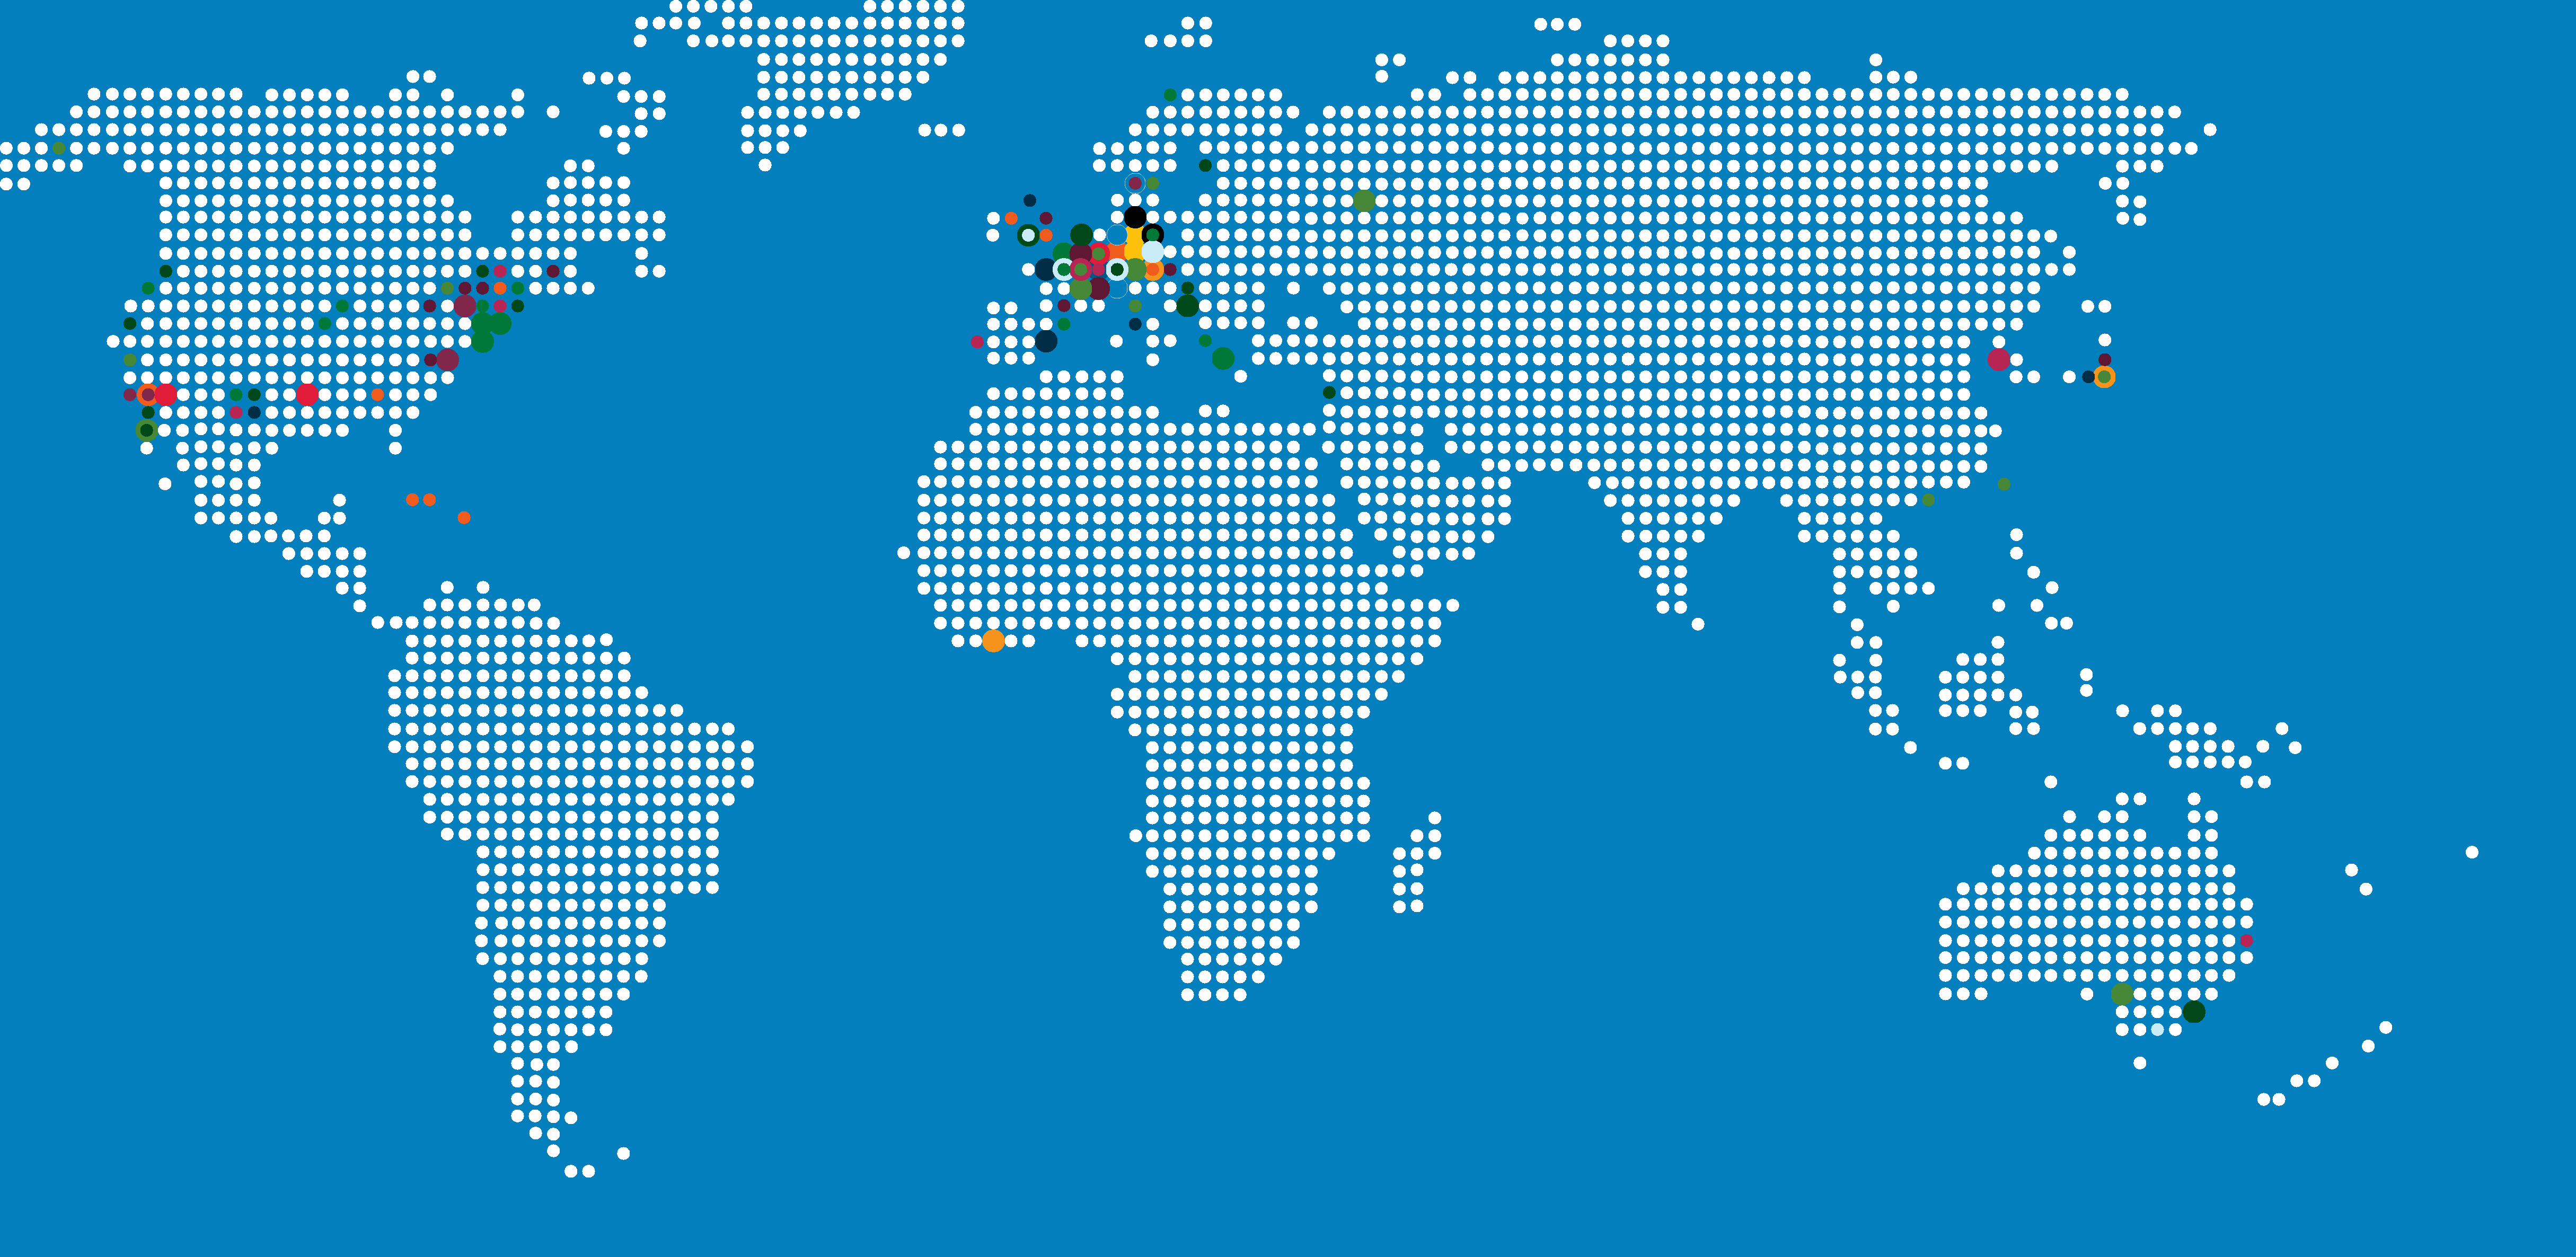
\includegraphics[width=.9\textwidth]{WORLDMAPDOTSdots.png}


Language Science Press m\"ochte die Oberhoheit \"uber den Publikationsprozess wieder in die H\"ande der sprachwissenschaftlichen Community legen. Dabei werden sowohl etablierte Wissenschaftler (Advisory Board, Reihenherausgeber) angesprochen, als auch Jungwissenschaftler (Community Proofreaders, Community Illustrators).  

	\begin{itemize} 
	    \item weltweite Autoren-, Leser- und Herausgeberschaft
	    \item weitl\"aufige Abdeckung der Subdisziplinen
	    \item 623 Supporter, 194 Editorial Board Members (siehe Karte), 165 Community Proofreader
	    \item \"uber 60.000 Downloads: Deutschland (20\,\%), China (13\,\%), USA (12\,\%), Ukraine (7\,\%), Frankreich (6\,\%), ...
	\end{itemize}  
}
    \end{block} 

    \setbeamercolor*{block title}{bg=lsp4}
    \begin{block}{Entwicklung}
	  \begin{itemize}
		      \item 20 Reihen, 26 publizierte B\"ucher, 204 Anfragen (10/2016)
	  \end{itemize} 
      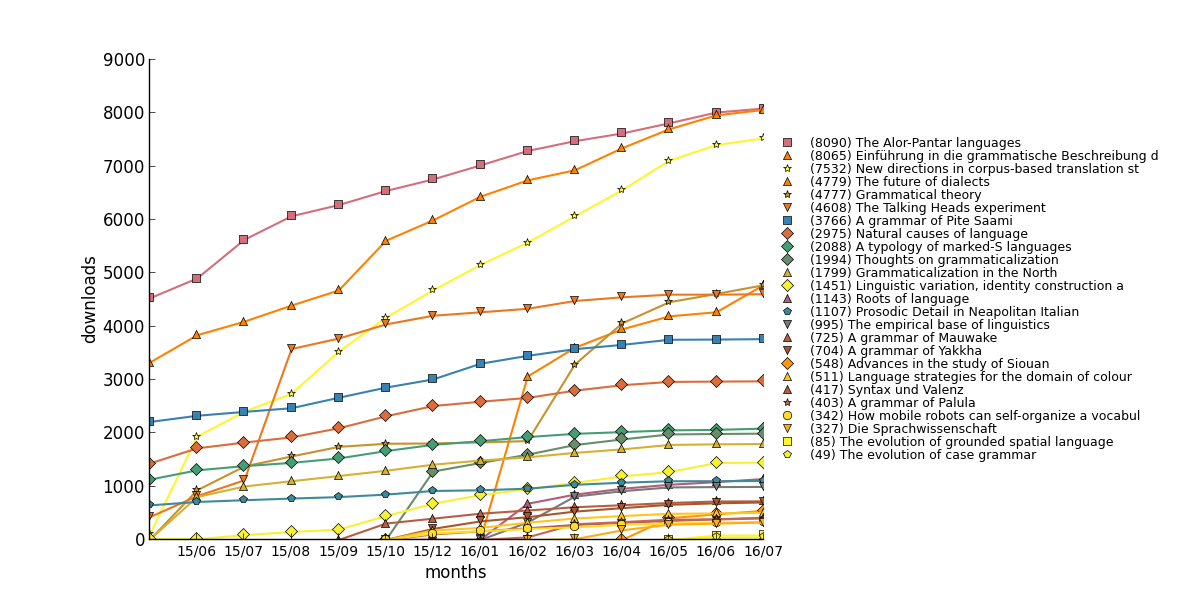
\includegraphics[width=.9\textwidth]{cumulativeall.png}
    \end{block}  
  

 

 

  \end{column}


  % bg=lsp2,3,4,5,6 etc f\"ur folgende K\"asten
  %%%%%%%%%%%%%%%%%%%%%%%%%%%%%%%%%%%%%%%%%%%%%%%%%%%%%%%%%%%%%%%%%%%%%%%%%%%%%%%%%%%%%%%%%%%%%%%%%%%%
% 				      Zweite Spalte
  %%%%%%%%%%%%%%%%%%%%%%%%%%%%%%%%%%%%%%%%%%%%%%%%%%%%%%%%%%%%%%%%%%%%%%%%%%%%%%%%%%%%%%%%%%%%%%%%%%%%
  \begin{column}{.45\linewidth}
    





    \setbeamercolor*{block title}{bg=lsp6}
    \begin{block}{Workflow} 
	\begin{enumerate} 
	    \item Webbasiert (Open Monograph Press) oder traditionell (E-Mail)
	    \item Bucherstellung mit {\LaTeX}
	    \item MS Word$\to${\LaTeX}-Webkonverter
	    \item Manuskriptfinalisierung mit Overleaf
	    \item ISBN, DOI, DOAB, OAPEN, GoogleBooks
	    \item Vertrieb \"uber print-on-demand (Taschenbuch: Createspace; gebunden: BoD). Gebundene B\"ucher sind auch \"uber den Buchhandel zu beziehen.
	\end{enumerate}  
     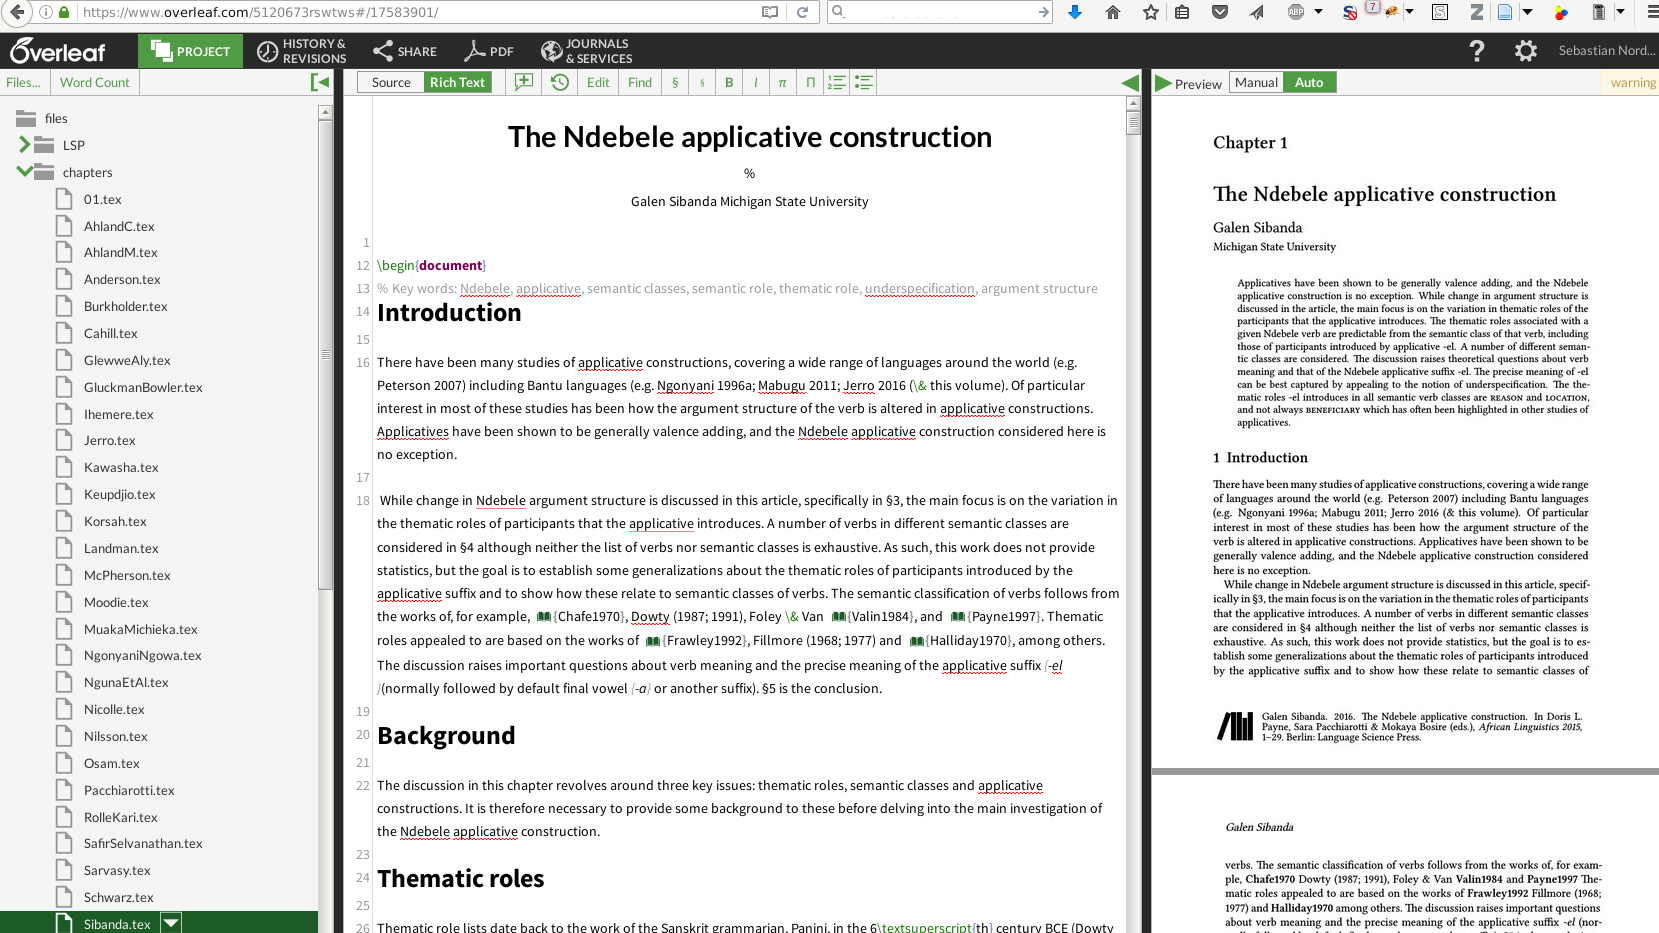
\includegraphics[width=.9\textwidth]{overleaf.png}
  
    \end{block} 



    \setbeamercolor*{block title}{bg=lsp7}
    \begin{block}{Reihen}
      \begin{columns}
	\begin{column}{.43\textwidth}
{\small
	  \begin{itemize}
\item African Language Grammars and Dictionaries 
 \item Classics in Linguistics  
 \item Computational Models of Language Evolution  
 \item Conceptual Foundations of Language Science 
 \item Contemporary African Linguistics   
 \item Em­pir­i­cal­ly Ori­ent­ed The­o­ret­i­cal Mor­phol­o­gy and Syn­tax 
 \item Eurosla Studies
 \item Im­ple­ment­ed Gram­mars  
	  \end{itemize}
}
	\end{column}
	\begin{column}{.53\textwidth}
{\small
	  \begin{itemize}
 \item Language Variation 
 \item Monographs on Comparative Niger-Congo  
 \item Morphological Investigations 
 \item Multiword Expressions and Phraseology
 \item Open Generative Syntax  
 \item Studies in Caribbean Languages  
 \item Studies in Diversity Linguistics  
 \item Studies in Laboratory Phonology  
 \item Textbooks in Language Sciences  
 \item Topics at the Grammar-Discourse Interface 
 \item Translation and Multilingual Natural Language Processing  \\
	  \end{itemize}
}
      \end{column}
      \end{columns}
      \vskip1ex 
    \end{block}
    
%     \setbeamercolor*{block title}{bg=lsp8}
%     \begin{block}{B\"{u}cher}
%       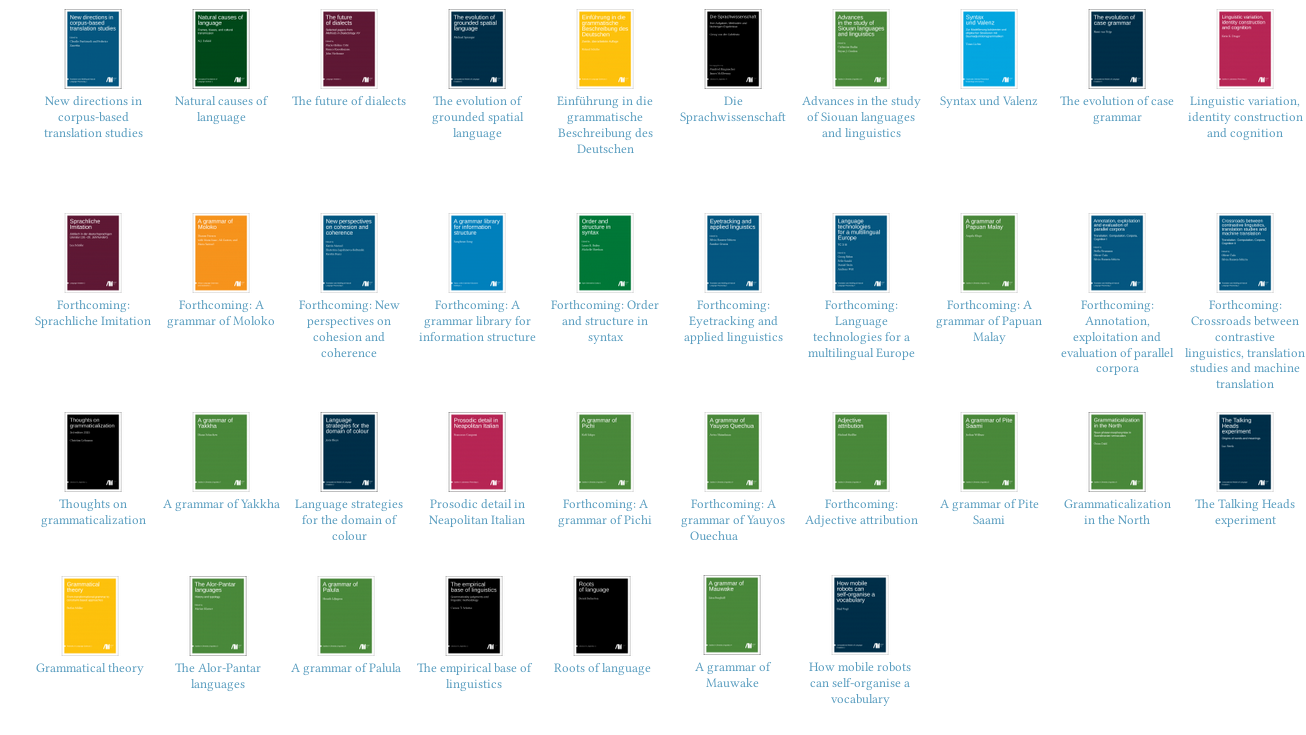
\includegraphics[width=.9\textwidth]{books.png}
%     \end{block}  
%   

    
    \setbeamercolor*{block title}{bg=lsp8}
    \begin{block}{Finanzierung} 
	\parbox{.9\textwidth}{
Eine F\"orderbedingung f\"ur die Anschubfinanzierung durch die DFG war die Erstellung eines Gesch\"aftsmodells durch eine Betriebswirtschaftlerin. Dieses Gesch\"aftsmodell liegt nun vor und ist auch die Basis des weiteren Betriebs an der HU. Es basiert auf folgenden Einnahmearten:
	\begin{enumerate} 
	    \item Printmarge
	    \item optionale Autorengeb\"uhren
	    \item institutionelle Mitgliedschaften \"uber Knowledge Unlatched
	    \item F\"ordermitglieder
	    \item Spenden
	\end{enumerate}  
}
    \end{block} 



    \setbeamercolor*{block title}{bg=lsp9}
    \begin{block}{Unterst\"utzer werden}

Language Science Press lebt von der Unterst\"utzung der Community: 
      \begin{columns}

	\begin{column}{.65\textwidth}
\begin{itemize}
 \item \"Offentliche Unterst\"utzung auf www.langsci-press.org/register
 \item Eintragen als Community Proofreader 
 \item Geldspende auf www.langsci-press.org/donate
 \item B\"ucher erwerben
 \item Werben eines institutionellen Mitglieds 
 \item Spread the word!
\end{itemize}

	\end{column}
	\begin{column}{.2\textwidth}
 
\includegraphics[width=\textwidth]{qrcode.png}
	\end{column}
\end{columns}
    
    \end{block}  
  \end{column}
  %%%%%%%%%%%%%%%%%%%%%%%%%%%%%%%%%%%%%%%%%%%%%%%%%%%%%%%%%%%%%%%%%%%%%%%%%%%%%%%%%%%%%%%%%%%%%%%%%%%%
  %%%%%%%%%%%%%%%%%%%%%%%%%%%%%%%%%%%%%%%%%%%%%%%%%%%%%%%%%%%%%%%%%%%%%%%%%%%%%%%%%%%%%%%%%%%%%%%%%%%%
\end{columns}
\vfill
\end{frame}

\end{document}


%%%%%%%%%%%%%%%%%%%%%%%%%%%%%%%%%%%%%%%%%%%%%%%%%%%%%%%%%%%%%%%%%%%%%%%%%%%%%%%%%%%%%%%%%%%%%%%%%%%%
%%% Local Variables: 
%%% mode: latex
%%% TeX-PDF-mode: t